\documentclass[12pt]{article}

\usepackage{../sbc/sbc-template}

\usepackage[english]{babel}
\usepackage[utf8]{inputenc}
\usepackage[T1]{fontenc}
\usepackage{amsmath, amssymb, graphicx, url}

\sloppy

\title{Computational Models Equivalent to Turing Machines\footnote{
    As submitted to the INE410113 class (Theory of Computation).}}

\author{Douglas Martins\inst{1}, Emmanuel Podestá Jr.\inst{1}, Gustavo
    Zambonin\inst{1}}

\address{
  Departamento de Informática e Estatística, Universidade Federal de Santa
    Catarina \\
  88040-900, Florianópolis, Brazil
  \email{\{marcelino.douglas,emmanuel.podesta,gustavo.zambonin\}@posgrad.ufsc.br}
}

\begin{document}

\maketitle

\section{Introduction}\label{sec:intro}

Solving problems is paramount to the advance of society, often being useful to
accelerate development in any area. By defining a finite number of instructions
that may produce outputs fully determined by respective inputs, one creates an
algorithm. This historic notion of an ``effective method'' for computations was
subsequently formalised independently by Church~\cite{Church:article:1936:apr},
with its $\lambda$-calculus, and Turing, through Turing
machines~\cite{Turing:article:1937:jan}. These models of computation are
equivalent and yield a class of functions known as computable functions.
Without loss of generality, these models can be thought of as some partial
functions on natural numbers, that is, $f : \mathbb{N}^{k} \rightarrow
\mathbb{N}$, such that any $k$-tuple will give $f(x)$ through an effective
method.

Note that this computational process may actually never stop, \emph{i.e.}
$f(x)$ may be an undefined value. It would be interesting to determine this
behaviour for any combination of algorithms --- or ``computer programs'' ---
and inputs. Called the halting problem, this was proved to be impossible to
solve through the Turing machine model of computation. It is not a computable
function, that is, there is no algorithm that accurately determines whether an
arbitrary algorithm will halt. The halting problem is frequently featured when
models are proven to be equivalent to Turing machines, and will aid to clarify
the reasoning behind these.

Models of computation that can simulate Turing machines are called
Turing-complete, or universal, and Turing-equivalent, if a Turing machine can
simulate that model. These definitions are the same in practice, since all
Turing-complete systems known are also Turing-equivalent (by the Church--Turing
thesis, this should remain the case for any computable functions). To
efficiently study models whose Turing-equivalence may not be obvious, we recall
the definition of a Turing machine and give descriptions of such models in
terms of these machines.

A Turing machine consists of a finite number of states, and features an
infinite one-dimensional tape divided into cells, each of which holds a symbol
from a finite tape alphabet. A tape head is always positioned at exactly one of
the cells, and can write to that cell, move to its left or right neighbours, or
order the machine to change states. The input, consisting of words from a
subset of the tape alphabet, is placed on the tape, each symbol in its own
cell, and all others initialised to blank, a special symbol from the tape
alphabet, and the tape head rests on the leftmost filled cell. The tape is
moved according to a series of instructions.

Formally, it is defined as a $7$-tuple $M = (Q, \Gamma, \Sigma, \delta, q_{0},
B, F)$, in which $Q$ is a finite, non-empty set of states, $\Gamma$ is a
finite, non-empty tape alphabet, $\Sigma \subset \Gamma$ is a non-empty input
alphabet, $B \in \Gamma, B \not\in \Sigma$ is the blank symbol, $q_{0} \in Q$
is the initial state, $F \subseteq Q$ is a set of accepting states, and $\delta
: (Q \: \backslash \: F) \times \Gamma \rightarrow Q \times \Gamma \times \{L,
R\}$ is the transition function, where $L, R$ are left and right shifts,
respectively. This last definition emulates the tape head movement.

With this definition in mind, note that the expressiveness of a Turing machine
is very reduced in comparison with \emph{e.g.} high-level general-purpose
programming languages. As such, even though a common program can theoretically
be represented and processed in a Turing machine, it may not be feasible to do
so. This is also the case in other models of computation. Still considering
such limitations, Turing-equivalent models may provide new insights into areas
of knowledge where a Turing machine is less suitable as an instrument to build
theories upon.

In this work, we present three models of computation and give proof ideas of
their Turing equivalence. Namely, we talk about cellular automata (a
$n$-dimensional grid of cells that change state according to their neighbours
own states at each discrete point in time), string rewriting systems (a binary
relation between strings over a finite alphabet), and non-deterministic
Diophantine machines (using Diophantine equations, multivariate polynomial
equations such that their roots are generated only by integers, as computing
devices).

\section{Cellular automata}\label{sec:ca}

In this section, we show a Turing-complete cellular automaton. More precisely,
a cellular automaton is a discrete model studied in several fields. The model
is composed by a $n$-dimensional cell grid, where each cell can have an
assortment of states. For each cell, we have a set of neighbours defined by
adjacent cells, and a value to characterise the initial configuration. In each
next configuration, called generation in this context, each cell value is
updated following a set of rules. These updates modify the state of a cell and,
as a result, have a new configuration.

In 1970, mathematician John Horton Conway created the Game of
Life~\cite{Gardner:article:1970:oct}. The game is a cellular automaton in a
bi-dimensional grid, and each cell show one of two possible states: alive ($1$)
or dead ($0$). Moreover, each cell follows a specific set of rules to change
between states. Therefore, for an initial configuration, or seed, cells change
their state without the necessity of user input.

\begin{figure}[h]
    \centering
    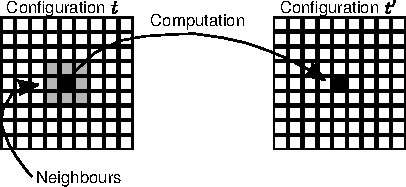
\includegraphics{images/stencil.pdf}
    \caption{Simplified cell state update.}
    \label{fig:stencil}
\end{figure}

Figure~\ref{fig:stencil} shows, in a simplified manner, how cell updates work.
For each cell, from a configuration $t$, a computation will be executed to
achieve a new state based on the cell neighbours. Therefore, we will have a new
configuration $t'$. More precisely, the game considers time as a discrete unit.
Hence, on a time $t'$, cells of the grid will have a state based on eight
adjacent cells from a time $t$ before $t'$. Moreover, when a cell turns alive
or dead on a time $t'$, we can define if that cell survived a new generation
(time step). The following rules are used to define the cell state in a
configuration $t'$, based on $t$:

\begin{itemize}
    \item An alive cell with less than two alive neighbours in $t$ will not
        survive the next generation, becoming a dead cell.
    \item An alive cell with two or three alive neighbours in $t$ will survive
        the next generation.
    \item An alive cell with more than three neighbours in $t$ will not
        survive.
    \item A dead cell with exactly three neighbours in $t$ will become alive.
\end{itemize}

Each of the aforementioned rules represents death by under-population,
sustainable life, death by over-population and birth, respectively. Therefore,
these rules represent the process of life and death.

There are several patterns that occur in Game of Life (GoL) that can be
classified based on their behaviour. Still life are patterns which can not be
modified between generations. Oscillators are patterns that return to their
initial state after a finite number of generations. Spaceships are patterns
that translate across the grid. More precisely, glider is a spaceship type
pattern, which interacts with other patterns in interesting ways. It is
possible to collide gliders, eliminating both from the next
generations~\cite{Adamatzky:book:2012}. Figure~\ref{fig:glider_gun} shows
another pattern, which generates gliders and propagates them across the grid,
appropriately named glider gun.

\begin{figure}[h]
    \centering
    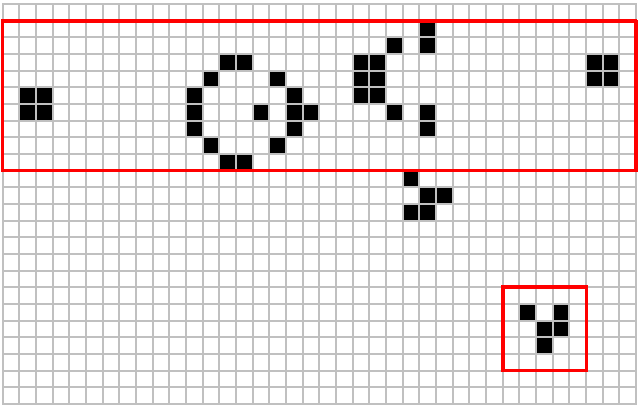
\includegraphics[scale=0.9]{images/glider-gun.pdf}
    \caption{Glider gun (upper rectangle) producing gliders (bottom
        rectangle).}
    \label{fig:glider_gun}
\end{figure}

Gliders and glider guns are patterns used to build logic ports, such as
\texttt{AND}, \texttt{OR} and \texttt{NOT}, and memory counters. Moreover,
glider gun patterns can produce live cells without boundaries. This
characteristic is interesting to computability, due to the fact that a
computational model is not Turing-complete, if it always stops. Hence, this
property implies, theoretically, that GoL is Turing-complete.

Rendell~\cite{Rendell:inproc:2011:jul, Rendell:phd:2014:jan} showed how to
build a Turing machine with Game of Life patterns.
Figure~\ref{fig:gol_mt_highlevel} illustrates the Turing machine diagram built
with the game. The machine has a finite state machine with stacks to represent
the states and tape, respectively. More precisely, the machine has two address
mechanisms, one for states and other for symbol value. Moreover, the machine
has nine memory cells. Each cell stores information about actions that can be
taken for each combination between state and symbol.

\begin{figure}[h]
    \centering
    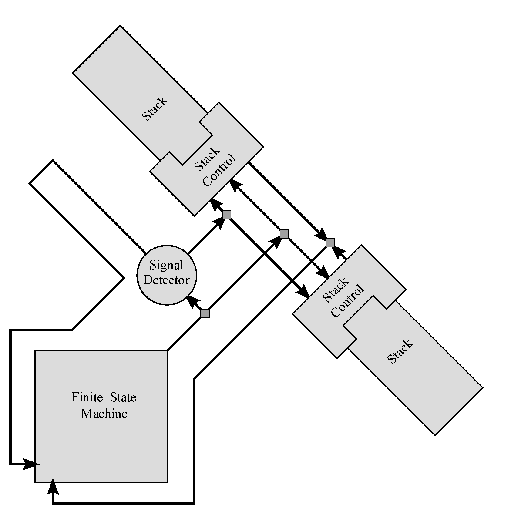
\includegraphics[width=0.75\textwidth]{images/gol-tm-high.pdf}
    \caption{Turing machine diagram. Original image by
        Rendell~\cite{Rendell:inproc:2011:jul}.}
    \label{fig:gol_mt_highlevel}
\end{figure}

The tape is portrayed with two stacks. In each cycle, stacks perform a push or
pop operation simultaneously. More precisely, these operations allow tape
movement. For example, if the right stack performs a pop operation, the element
removed will be redirected to the finite state machine. The machine will
compute and produce an output. On the other hand, the left stack will perform a
push operation with the output from the finite state machine. These operations
characterise a right movement on the tape. The left movement can be achieved
with the same process. Finally, all the signal and stack control are made by
the Stack Control component.

The Signal Detector component collects and distributes output information from
the finite state machine to necessary places. The component splits the next
state information from the output, and sends it to the machine. This
information is used by the finite state machine in the next read/write cycle.
The information about the next state and the symbol arrival must be
synchronised. Information about the symbol value is collected by the pop
operation.

The Turing machine was built with logic gates manually. All memory, stacks,
signal and other elements were implemented explicitly with the game. Moreover,
word input and initial tape is made, also, explicitly with binary signals.
Figure~\ref{fig:gol_mt} shows the Turing machine built through the cellular
automaton. Therefore, we can simulate a Turing machine with Game of Life,
characterising the Turing-completeness of the game.

\begin{figure}[h]
    \centering
    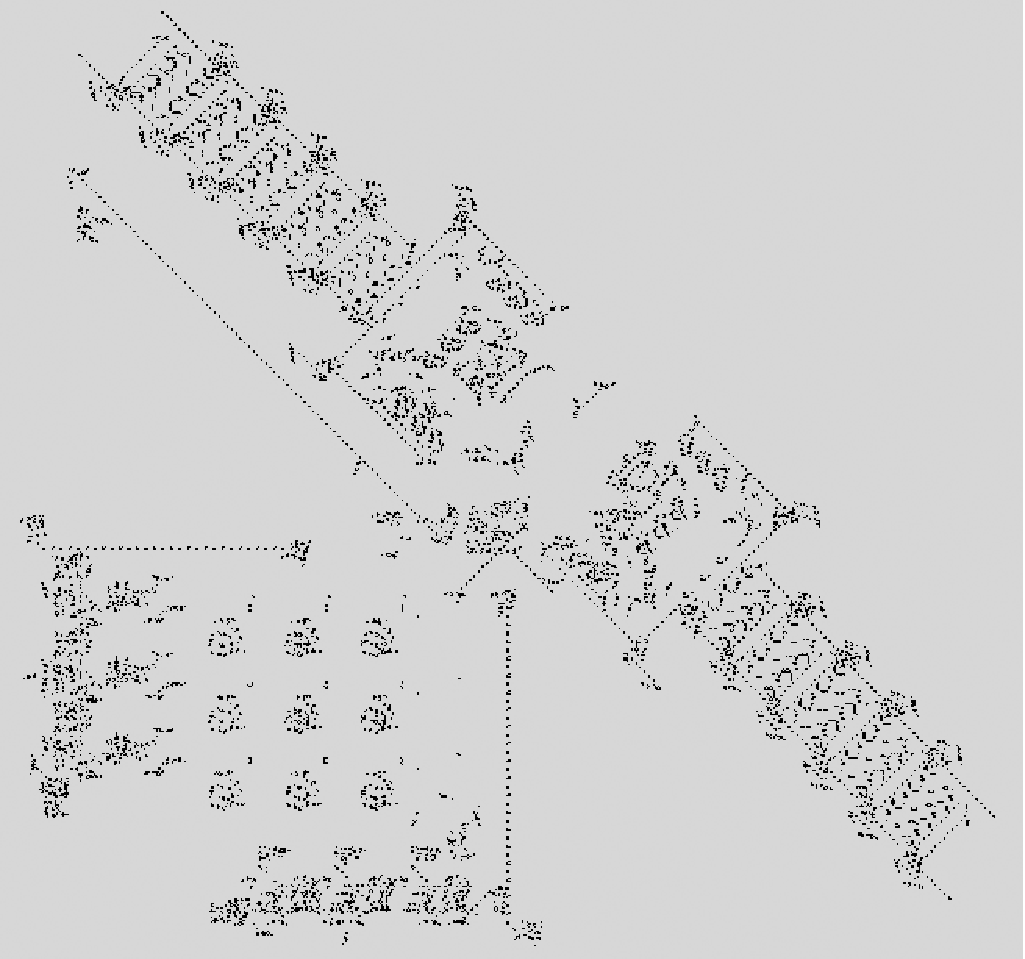
\includegraphics[width=0.6\textwidth]{images/gol-tm.pdf}
    \caption{Patterns used in the Turing machine. Original image by
        Rendell~\cite{Rendell:inproc:2011:jul}.}
    \label{fig:gol_mt}
\end{figure}

On the other hand, we want to simulate GoL with a Turing machine. To accomplish
this objective, we can build a multi-tape Turing machine, where each tape
represents a line in a bi-dimensional grid. Recall that a multi-tape Turing
machine is equivalent to a single-tape Turing machine~\cite[Theorem
3.13]{Sipser:book:2012}. Consider the computation of a element $c$ on tape $t$.
The head of $t$ will move to evaluate neighbours of $c$. Moreover, heads from
other tapes will move accordingly to evaluate neighbours from different lines.
After the evaluation, we can change the value in $c$. Hence, we can move the
head of each tape and transition between states based on rules of the game.
Freely moving the head of each tape allows the change of each cell based on
neighbours from any tapes.

More precisely, we can define a 7-tuple M = ($Q$, $\Gamma$, $\Sigma$, $\delta$,
$q_0$, $B$, $F$), whose Q is a finite, non-empty set of states; $\Gamma$ is a
finite, non-empty tape alphabet; $\Sigma \in \{0, 1\}$ and $\Sigma \subset
\Gamma$; $B \in \Gamma$ is the blank symbol; $q_0 \in Q$ is the initial state
and $F \subseteq Q$ is a set of accepting states. Tapes will have an initial
configuration with values from the alphabet. The heads will move across the
tapes to simulate a sweep on the matrix. Moreover, $\delta$ will be the
transactions based on the rules of the game. Therefore, we can simulate GoL
with a Turing nachine.

The Game of Life may be used in several applications, mainly in non linear
system models in physics, mathematics, biology and other fields. More
precisely, a cellular automaton can be used in a private-public
cryptosystem~\cite{Guan:article:1987:feb}. Hence, we can represent a set $S$ of
bits as a field or ring. The rules used by the automaton may be represented as
polynomial functions, allowing the definition of addition and multiplication
over elements of $S$. Moreover, cellular automata may be used to generate
pseudo-random integers~\cite{Wolfram:article:1986:jun}.

\section{String rewriting systems}\label{sec:srs}

When studying formal systems, it is natural to think about how elements (or
terms) of these systems can be expressed in other, more useful, forms.
Algebraic expressions or logic propositions may be represented in a different
way, according to rules given by the system, in the form of axioms and
inferences. For instance, in formal grammars, these terms are usually strings
over an alphabet, that may be members of a language. Within this context, it is
very intuitive to think of these rules as string transformations. To restrict
or alter behaviour in specific ways, the notions of terminals, non-terminals,
productions and other intricacies are enforced. Thus, it is a common example of
a string rewriting system (SRS) in formal language theory.

Let us formally define a SRS. This definition is taken from Book and
Otto~\cite[Sec. 2.1]{Book:book:1993}. Consider $\Sigma$ to be a finite set of
symbols, that is to say, an alphabet, and a binary relation $R \subseteq
\Sigma^{*} \times \Sigma^{*}$. A string rewriting system is a $2$-tuple $S =
(\Sigma, R)$. Any member $x \in R$ is called a rewrite rule. Further, take any
words $u, v, x, y \in \Sigma^{*}$ and define the single-step reduction relation
$u \rightarrow_{R} v$, if and only if there exists a pair $(l, r) \in R$ such
that $u = xly$ and $v = xry$. This enables any substring to be rewritten
according to the rules of $S$. The reduction relation $u
\stackrel{*}{\rightarrow}_{R} v$ is the reflexive transitive closure of
$\rightarrow_{R}$, that represents all substrings that can be created by an
initial string. Evidently, this closure may be finite or infinite.

This formalism is historically known as a semi-Thue system, and was first
defined by Thue~\cite{Thue:article:1914:may}\footnote{This work was translated
to English by Power~\cite{Power:misc:2013:aug}.}. It is abstract enough to
represent other definitions, for instance, that of a free monoid in abstract
algebra. To show that it is equivalent to a Turing machine, we will follow the
reasoning presented by Davis~\cite{Davis:book:1958}. Afterwards, we show that a
handful of constructions are directly related to string rewriting systems. We
will present succinct definitions for Post canonical systems and tag systems,
with the intent of constructively showing that a SRS has many special cases or
equivalent definitions.

For the first step, a possible proof strategy is based on showing that a
general SRS is a recursively enumerable (r.e.) language, that is,
Turing-recognizable. Indeed, it is a formal language. Then, one must prove that
a SRS generates a set of outputs that is a r.e. subset of the set of all
possible words over its alphabet. This means that there exists an algorithm
which enumerates the members of that subset. Equivalently, there exists a
Turing machine that will enumerate all valid strings of the
language~\cite[Theorem 3.21]{Sipser:book:2012}. This is shown to be true by
Davis~\cite[pp. 84--86]{Davis:book:1958} (esp. Theorem 1.5), by means of
representing sets of strings generated by a language as Gödel numbers, a
special encoding based on prime factorisation that helps in working with
partial functions.

Secondly, we must now translate Turing machines into string rewriting systems.
We quote an introduction by Davis~\cite[Sec. 6.2]{Davis:book:1958} on the
rationale behind this conversion.

\begin{quote}
    Next, we shall show how the theory of simple Turing machines can be
    interpreted (at least for certain purposes) as a part of the theory of
    semi-Thue systems. With each simple Turing machine $Z$ and integer $m$ we
    shall associate a semi-Thue system $\tau_{m}(Z)$, designed to imitate the
    behaviour of the simple Turing machine $Z$ at the instantaneous description
    $q_{1}\overline{m}$. That is, the theorems of $\tau_{m}(Z)$ are to
    correspond roughly to the successive instantaneous descriptions of $Z$.
\end{quote}

Recall that semi-Thue systems are the historical name of string rewriting
systems. Evidently, theorems from a SRS are outputs from successive string
rewrites given an input. A ``simple'' Turing machine definition~\cite[Sec. 1.1,
Def. 1.3]{Davis:book:1958} is straightforward, only instead of quintuples,
Davis uses quadruples to represent actions of the machine. ``Instantaneous
descriptions'' are what we call states. The proof is given shortly after the
introduction~\cite[pp. 88--93]{Davis:book:1958}.

First, Davis proves a handful of lemmas about a specifically constructed SRS,
with the intent of showing Theorem 2.2, that formally describes the machine
constructed from the SRS, according to the strategy above, independent of the
integer $m$. In special, it is noted that all rules in the SRS need to be
inverted. This is taken into account for the next lemmas, that culminate in
Theorem 2.4, which states that ``every recursively enumerable set is generated
by a semi-Thue system''. Hence, it is proven that string rewriting systems and
Turing machines are equivalent. Remarkably, the word problem for semi-Thue
systems, that asks if it is possible to know whether a word from the alphabet
can be generated from another using rules from the system, is equivalent to the
halting problem.

A more tangible example is given by Hamel~\cite{Hamel:misc:2016:sep}.
Informally, consider a Turing machine in which its tape is divided in three
parts, marked with special symbols. The first part holds the input string, and
the second part contains the rules for the SRS. The third part is initially
empty and serves as a scratchpad for eventual partial computations. To process
the input, the machine should try to match the leftmost symbols of the input
string with the left sides of rules in the second tape, and substitute them as
described by the right side of the earliest matched rule. When no further
matching is possible, the computation stops.

Conversely, we want string rewriting systems to emulate Turing machines. We
will create sets of rules, divided into those that can move the tape head
forwards, or backwards, or actual calculations upon the input string. Of
course, we need to signal where the input begins and ends, current position of
the tape head and state information with special symbols. Hence, we will have a
list of rules that acts on a partial string that represents a pseudo-tape.
Indeed, these sets of rules will be finite, since they are equivalent to the
description of possible transitions in a Turing machine. Formally, an example
of this construction was created by Book and Otto~\cite[Sec.
2.5]{Book:book:1993}.

Now, we turn to examples of equivalent definitions for string rewriting
systems. We start with Post canonical systems. This definition is taken from
Minsky~\cite[Sec. 12.5]{Minsky:book:1967}. Let $\Sigma$ be a finite alphabet,
$X$ be a set of axioms composed of strings from the alphabet, and a set of
productions $P$ of the form $u \rightarrow v$, where $u =
g_{0}\$_{1}g_{1}\$'{1} \dots \$_{n}g_{n}$ is the antecedent and $v =
h_{0}\$'_{1}h_{1}\$'_{1} \dots \$'_{n}h_{n}$ is the consequent. For $i = \{0,
\dots, n\}$, $g_{i}, h_{i} \in \Sigma^{*}$, and $\$_{i}$ are called variables,
that have to be replaced by their respective $\$'_{i}$. These variables are
also words from the alphabet.

Hence, a Post canonical system is a $3$-tuple $\mathcal{P} = (\Sigma, X, P)$,
with the restrictions above. If each $p \in P$ has the form $g\$ \rightarrow
\$h$ with $g, h, \$ \in \Sigma^{*}$, $\mathcal{P}$ is a Post normal system. We
can see that every production in a Post canonical system can be split into
smaller productions. Indeed, Post normal systems are equivalent to their
canonical counterparts~\cite[Theorem 13.1]{Minsky:book:1967}. We can then use
this result to demonstrate that Post normal systems are in fact equivalent to
string rewriting systems~\cite[Sec. 6.5, Theorem 5.1]{Davis:book:1958}.
Additionally, a direct proof for the equivalence of Turing machines and Post
canonical systems is also given by Minsky~\cite[Sec. 12.6]{Minsky:book:1967}.

\emph{Example.~\cite[Problem 12-4.3]{Minsky:book:1967}} Let a Post canonical
system $\mathcal{P} = (\Sigma, X, P)$ that describes multiplication of unary
strings, such that $\Sigma = \{1, \times, =\}, X = \{1 \times 1 = 1\}, P =
\{p_{1}, p_{2}\}$, where
\begin{align}
    p_{1} = \$_{1} \times \$_{2} = \$_{3} &\rightarrow \$_{1}1 \times \$_{2}
        = \$_{3}\$_{2}, \label{eq:p1} \\
    p_{2} = \$_{1} \times \$_{2} = \$_{3} &\rightarrow \$_{2} \times \$_{1}
        = \$_{3}. \label{eq:p2}
\end{align}
Let us compute $3 \times 4 = 12$, or rather, the unary string representing this
operation.
\begin{align}
    1    \times 1    &= 1            \label{eq:1} \\
    11   \times 1    &= 11           \label{eq:2} \\
    111  \times 1    &= 111          \label{eq:3} \\
    1111 \times 1    &= 1111         \label{eq:4} \\
    1    \times 1111 &= 1111         \label{eq:5} \\
    11   \times 1111 &= 11111111     \label{eq:6} \\
    111  \times 1111 &= 111111111111 \label{eq:7}
\end{align}
Observe that Eq.~\ref{eq:1} is given by the only axiom in $X$. We apply
Eq.~\ref{eq:p1} in Eqs.~\ref{eq:2},~\ref{eq:3} and~\ref{eq:4}, to expand the
first and last variables. Eq.~\ref{eq:5} swaps the terms around by means of
Eq.~\ref{eq:p2} and Eqs.~\ref{eq:6} and~\ref{eq:7} use Eq.~\ref{eq:p1} again to
carry out the remaining multiplications.

A special case of Post normal systems are tag systems, where productions have
special restrictions. This definition is due to Minsky~\cite[Sec.
14.6]{Minsky:book:1967}. Namely, all antecedents have the same length $n$ and
all consequents depend only on the first letter of its respective antecedent.
By virtue of these characteristics, it is helpful to think about how to use
such a system. The first letter for the string being operated is read and an
appropriate production chosen. Then, its first $n$ letters are deleted, and the
consequent for the chosen production is appended to the end of the string. For
completeness, we note that a proof of equivalence between tag systems and
Turing machines is given by Minsky~\cite[Theorem 14.6-1]{Minsky:book:1967}.

\emph{Example.~\cite[Theorem 2.1]{DeMol:article:2008:nov}} a tag system
$\mathcal{T} = (\Sigma, X, P)$, with $n = 2, \Sigma = \{\alpha, \beta,
\gamma\}, X = \{\alpha^{k} \mid k \in \mathbb{N}^{*}\}, P = \{p_{1}, p_{2},
p_{3}\}$. The Collatz conjecture asks if, for any positive integer, repeated
applications of
\begin{align}
    f(n) =
    \begin{cases}
        \frac{n}{2} & \text{if } n \equiv 0 \pmod{2}, \\
        3n + 1      & \text{if } n \equiv 1 \pmod{2}
    \end{cases}
\end{align}
eventually reaches $1$. Collatz sequences are the list of numbers generated by
this process. Also, note that the axioms are now all non-negative natural
numbers, expressed in unary form. The production rules for the generation of
such sequences are given as follows:
\begin{align}
    p_{1} = \alpha &\rightarrow \beta\gamma,        \\
    p_{2} = \beta  &\rightarrow \alpha,             \\
    p_{3} = \gamma &\rightarrow \alpha\alpha\alpha.
\end{align}
These rules actually compute $\frac{3n + 1}{2}$ if $n$ is odd, giving a more
efficient calculation of the sequence. Still, without loss of generality, let
us compute the Collatz sequence for $k = 5$, which is $\{5, 8, 4, 2, 1\}$.
\begin{align}
    \boldsymbol{\alpha\alpha\alpha\alpha\alpha},
        \quad \alpha\alpha\alpha\beta\gamma,
        \quad \alpha\beta\gamma\beta\gamma,
        \quad \gamma\beta\gamma\beta\gamma,
        \quad \gamma\beta\gamma\alpha\alpha\alpha,
        \quad \gamma\alpha\alpha\alpha\alpha\alpha\alpha, \\
    \begin{split}
        \boldsymbol{\alpha\alpha\alpha\alpha\alpha\alpha\alpha\alpha},
            \quad \alpha\alpha\alpha\alpha\alpha\alpha\beta\gamma,
            \quad \alpha\alpha\alpha\alpha\beta\gamma\beta\gamma,
            \quad \alpha\alpha\beta\gamma\beta\gamma\beta\gamma, \\
            \quad \beta\gamma\beta\gamma\beta\gamma\beta\gamma,
            \quad \beta\gamma\beta\gamma\beta\gamma\alpha,
            \quad \beta\gamma\beta\gamma\alpha\alpha,
            \quad \beta\gamma\alpha\alpha\alpha, &
    \end{split} \\
    \boldsymbol{\alpha\alpha\alpha\alpha},
        \quad \alpha\alpha\beta\gamma,
        \quad \beta\gamma\beta\gamma,
        \quad \beta\gamma\alpha, \\
    \boldsymbol{\alpha\alpha},
        \quad \beta\gamma, \\
    \boldsymbol{\alpha}.
\end{align}
Strings in bold are elements of the Collatz sequence. Note that computation
stops when the length of the string is less than $n$, since no more symbols can
be deleted.

We cannot help but list various other formalisms such as Markov algorithms,
cyclic tag systems, unrestricted grammars etc., that are equivalently powerful
and defined in term of string rewriting systems. In special, an one-dimensional
cellular automaton known as Rule 110 is proven Turing-equivalent through
conversion to cyclic tag systems by Cook~\cite{Cook:article:2004:mar}. Finally,
string rewriting systems define a rather abstract idea of string modifications,
encompass various definitions, and are very helpful in equivalence proofs, as
seen above, as well as allowing a simple description of languages.

\section{Non-deterministic Diophantine machines}\label{sec:nddm}

Connections between areas of mathematics are quite common, allowing researchers
to reuse and adapt existing knowledge to other, possibly very distinct
concepts. Since theoretical computer science is evidently a branch of
mathematics, it is expected that such translations are to occur within this
subset. Hence, it is likely that results from pure mathematics affect computer
science or vice-versa, or that computational approaches may help with more
abstract notions. Indeed, the very first computer scientists were originally
mathematicians. In this section, we will see how a result from number theory
connects with ideas of computability theory, and gives rise to a curious
formalism equivalent to Turing machines.

In the year 1900, Hilbert famously posed a list of 23 interesting mathematical
problems~\cite{Hilbert:article:1900:dec}\footnote{Translated by
Newson~\cite{Hilbert:article:1902:jul}.}, which were at the time unsolved.
Although their descriptions are simple, they have eluded many mathematicians
since their publication. We will focus on the tenth problem, a number-theoretic
question that is enunciated as follows.

\begin{quote}
    Given a Diophantine equation with any number of unknown quantities and with
    rational integral numerical coefficients: to devise a process according to
    which it can be determined by a finite number of operations whether the
    equation is solvable in rational integers.
\end{quote}

In modern words, it is asked for an algorithm that can decide if, for any
possible Diophantine equation, it has a solution comprised only of integers. To
understand this question and draw the appropriate parallels between mathematics
and computability theory, we first need to define Diophantine equations and
other helpful notions.

A Diophantine equation is a multivariate polynomial with integer coefficients,
\emph{i.e.}
\begin{align}
    D(x_{1}, x_{2}, \dots, x_{n}) = 0, \qquad n \in \mathbb{N}^{*},
        \label{eq:d1}
\end{align}
such that only integral solutions are considered, that is, all variables must
be integers. Examples are the Pythagorean equation $a^{2} + b^{2} = c^{2}$, or
Bézout's identity $ax + by = d$. Note that variables can appear as exponents,
in which case an exponential Diophantine equation occurs. Generalising this
concept, a family of Diophantine equations is given by
\begin{align}
    D(a_{1}, \dots, a_{m}, x_{1}, \dots, x_{n}) = 0, \qquad m, n \in
        \mathbb{N}^{*}, \label{eq:d2}
\end{align}
where all $a_{i}$ are called variables and all $x_{i}$ are called unknowns.
Note that it may be the case where a set of variables does not give rise to a
Diophantine equation with a valid solution. Further, a set $S$ consisting of
$m$-tuples of variables that satisfy Eq.~\ref{eq:d2} in its unknowns, that is,
\begin{align}
    (a_{1}, \dots, a_{m}) \in S \Leftrightarrow \exists (x_{1}, \dots, x_{n})
        \text{ s.t. } D(a_{1}, \dots, a_{m}, x_{1}, \dots, x_{n}) = 0,
\end{align}
is called a Diophantine set. The set of Pythagorean triples is Diophantine, as
is the set of natural numbers, prime numbers~\cite{Jones:article:1976:jun}, and
many others. In fact, we will see that these sets can be thought of entirely as
other concepts.

With these definitions in mind, we may look at how the question of Hilbert was
solved. First, note that all Diophantine sets are recursively enumerable, since
a Turing machine can enumerate all possible pairs of variables and unknowns and
then test if they are valid solutions to a equation. However, are all r.e. sets
also Diophantine, that is, can a Turing machine decide whether a Diophantine
equation can be solved? This statement was answered negatively by the
Davis--Putnam--Robinson--Matiyasevich
theorem~\cite{Matiyasevich:article:1970:jun}, and it is another formulation of
the halting problem. In other words, Diophantine equations have the same
computational power as Turing machines.

We will follow the proof idea due to Matiyasevich~\cite[Chap.
5]{Matiyasevich:book:1993}, which is easier to follow than the original
strategy. Usual definitions of Turing machines and their composability are
given in Sections 5.1 and 5.2, respectively. Two special symbols for the
beginning of tape and empty value are used, as well as four alphanumeric
symbols representing unary words, delimiters and markers, to compose the total
alphabet. All machines used are deciders, in the sense that their only final
states are ``yes'' or ``no''. Chaining and looping of machines is also
explained in the customary way.

In Section 5.3, various machines are built from this definition. Simple tape
actions, like moving to the left or right, reading or writing to a cell are
first defined. More complex movements, such as moving to a specific cell
depending on its contents, are also defined. Afterwards, operations that deal
with tuples of elements are given: increment, decrement, deletion, marking,
concatenation, comparison, addition and multiplication of symbols. These
notations all come together in Section 5.4, where it is shown that, indeed,
Turing machines recognise Diophantine sets. Thus, these two sections are a
formal definition of the process given above.

Section 5.5 then establishes that sets encoding Turing machines, that is, r.e.
sets, are Diophantine. This is done as follows. Each state of a Turing machine
is represented as a configuration tuple of integers, consisting of the current
tape contents, state, and head position. These are encoded such that they
uniquely determine the current configuration for the machine, and are
represented as a Diophantine equation. Then, it is proved that an atomic change
of configuration generates a new valid equation, through careful translation of
the Turing machine transition functions to Diophantine representations (see
Eqs. 5.5.7 and 5.5.15).

The argument above is generalised to the execution of multiple steps by the
Turing machine. By means of concatenating all intermediate configurations, a
superconfiguration is created, that describes the operation of a supermachine,
with multiple heads and tapes, operating in accordance with the original
machine. After determining several results on the uniqueness and behaviour of
these equations and asserting that they are Diophantine, it is thus proved that
any Turing machine has an equivalent Diophantine representation. Finally,
Section 5.6 gives an argument on the unsolvability of the halting problem
through the lenses of these equations.

To further illustrate the concept of Diophantine equations as general problem
solvers, we show the notion of non-deterministic Diophantine machines. Due to
Manders and Adleman~\cite[Sec. 3]{Manders:article:1978:apr}, this definition
was presented much earlier than the proof showed above. Still, it captures
intuitively the processing power of Diophantine equations through equivalence
to non-deterministic Turing machines. Recall that non-deterministic Turing
machines are as powerful as their deterministic counterparts~\cite[Theorem
3.16]{Sipser:book:2012}. Consider Eq.~\ref{eq:d2}, and let the machine work as
follows: input the tuple of variables $(a_{1}, \dots, a_{m})$ and
non-deterministically guess tuples of unknowns $(x_{1}, \dots, x_{n})$. If a
root is found, then accept the corresponding tuple of variables. For instance,
if the equation is $a_{1} - x_{1}^{2} = 0$, then the machine naturally decides
whether a number is a perfect square.

Obscure equivalent definitions of Turing machines may certainly be well-known
problems in other areas, as is the case with the tenth problem of Hilbert. It
is thus interesting to look at non-deterministic Diophantine machines as tools
to solve problems in number-theoretic contexts, where the introduction of a
computational device such as a Turing machine may be unfit. Further, the
theoretical result stating that all r.e. sets are Diophantine is a
ground-breaking result on its own. Hence, Diophantine equations are certainly
useful, if not curious, computational models.

\section{Conclusion}\label{sec:conc}

Throughout this work, we have seen several definitions of computational models
that are equivalent to Turing machines. Namely, a peculiar cellular automaton
called Game of Life, abstractions of formal grammars called string rewriting
systems, and number-theoretic non-deterministic Diophantine machines. Several
other mathematical definitions exist, such as Markov algorithms, queue
automata, one-instruction set computers, Post machines, register machines and
$\mu$-recursive functions. Curiously, if we ignore the infinite memory
restriction, most programming languages and even some video games are
Turing-complete, in the imprecise sense. We have learned that simple equations
actually represent all possible Turing machines, that a fun zero-player game
can be commanded to act as a digital
clock\footnote{\url{https://codegolf.stackexchange.com/a/111932}}, and that
every algorithm can be characterised as plain string transformations. This is
useful in the sense that one can abuse this behaviour to exploit computation in
various disciplines, without boundaries that perhaps could be solved by another
model.

\bibliographystyle{../sbc/sbc}
\bibliography{ref}

\end{document}
